\begin{center}
    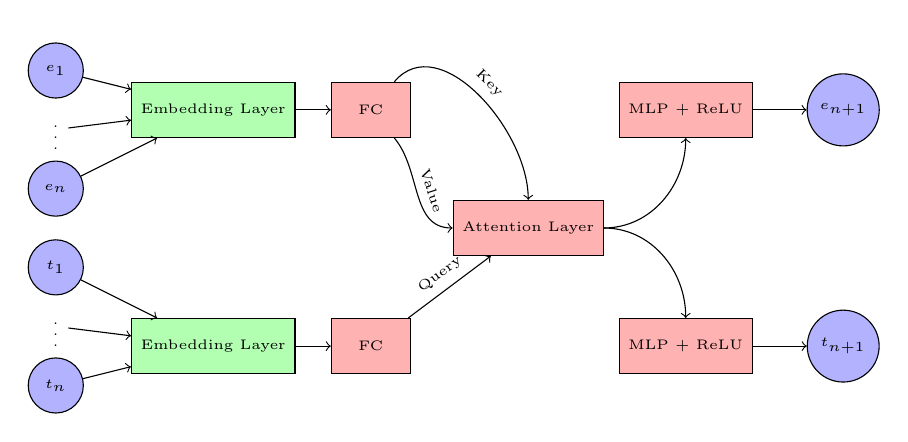
\begin{tikzpicture}[
            neuron/.style={circle, draw, minimum size=0.7cm},
            rect neuron/.style={rectangle, draw, minimum width=1cm, minimum height=0.7cm}, % Rectangular neuron
            input neuron/.style={neuron, fill=blue!30},
            embeddings neuron/.style={rect neuron, fill=green!30},
            mlp neuron/.style={rect neuron, fill=red!30},
            output neuron/.style={neuron, fill=red!30},
            every node/.style={align=center,font=\tiny}
    ]
        % Input Layer
        \node[input neuron] (inp_e1) at (0,2) {$e_1$};
        \node (other_e) at (0, 1.25) {\vdots};
        \node[input neuron] (inp_e2) at (0,0.5) {$e_n$};
        \node[input neuron] (inp_t1) at (0,-0.5) {$t_1$};
        \node (other_t) at (0, -1.25) {\vdots};
        \node[input neuron] (inp_t2) at (0,-2) {$t_n$};
        % Text Processing

        \node[embeddings neuron] (emb_e) at (2,1.5) {Embedding Layer};
        \node[embeddings neuron] (emb_t) at (2,-1.5) {Embedding Layer};

        % Emotion Processing
        \node[mlp neuron] (MLP1_emo) at (4,1.5) {FC};
        \node[mlp neuron] (MLP1_txt) at (4,-1.5) {FC};

        \node[mlp neuron] (attn) at (6,0) {Attention Layer};
        % Final Emotion

        \node[mlp neuron] (MLP2_emo) at (8,1.5) {MLP + ReLU};
        \node[mlp neuron] (MLP2_txt) at (8,-1.5) {MLP + ReLU};

        \node[input neuron] (out_emo) at (10,1.5) {$e_{n+1}$};
        \node[input neuron] (out_txt) at (10,-1.5) {$t_{n+1}$};

        % Arrows
        \draw[->] (inp_t1) -- (emb_t);
        \draw[->] (other_t) -- (emb_t);
        \draw[->] (inp_t2) -- (emb_t);
        \draw[->] (emb_t) -- (MLP1_txt);
        \draw[->] (MLP1_txt) -- (attn) node[pos=0.5,,sloped,above] {Query};

        \draw[->] (inp_e1) -- (emb_e);
        \draw[->] (other_e) -- (emb_e);
        \draw[->] (inp_e2) -- (emb_e);
        \draw[->] (emb_e) -- (MLP1_emo);
        \draw[->] (MLP1_emo) to[out=50,in=90] node[above,sloped] {Key} (attn);
        \draw[->] (MLP1_emo) to[out=-50,in=180] node[above,sloped] {Value} (attn);
        
        \draw[->] (attn) to[out=0,in=-90] (MLP2_emo);
        \draw[->] (attn) to[out=0,in=90] (MLP2_txt);

        \draw[->] (MLP2_emo) -- (out_emo);
        \draw[->] (MLP2_txt) -- (out_txt);

    \end{tikzpicture}
\end{center}

